
% !TeX spellcheck = de_DE
\documentclass{article}

\usepackage[ngerman]{babel}
\usepackage{graphicx}
\usepackage{float}
\usepackage{booktabs}
\usepackage{lscape}
\usepackage{longtable}

\graphicspath{ {./images/} }
\setlength\parindent{0pt}

\setlength\LTleft{0pt}
\setlength\LTright{0pt}

\makeatletter
\newcommand{\sectionauthor}[1]{
	{\parindent 0em \large \scshape Autor: #1 \par \nobreak \vspace*{1em}}
	\@afterheading
}
\newcommand{\specification}[3]{
	{\parindent 0.5em \hangindent 3em \hypertarget{spec:#1:#2}{\textbf{/#1#2/}} #3 \par \nobreak \vspace*{0.5em}}
}
\makeatother

\title{Bibliotheksanwendung - Feinspezifikation}
\date{\today\\v1.1}
\author{
	Ivan Charviakou\\
	León Liehr\\
	Mohamad Najjar\\
	Jonas Picker\\
	Sergei Pravdin
}

\begin{document}

%--Titel----------------------------------------------------------------------------------------------------------------------------------------------------------------------------------
\maketitle
\begin{figure}[H]
	\centering
	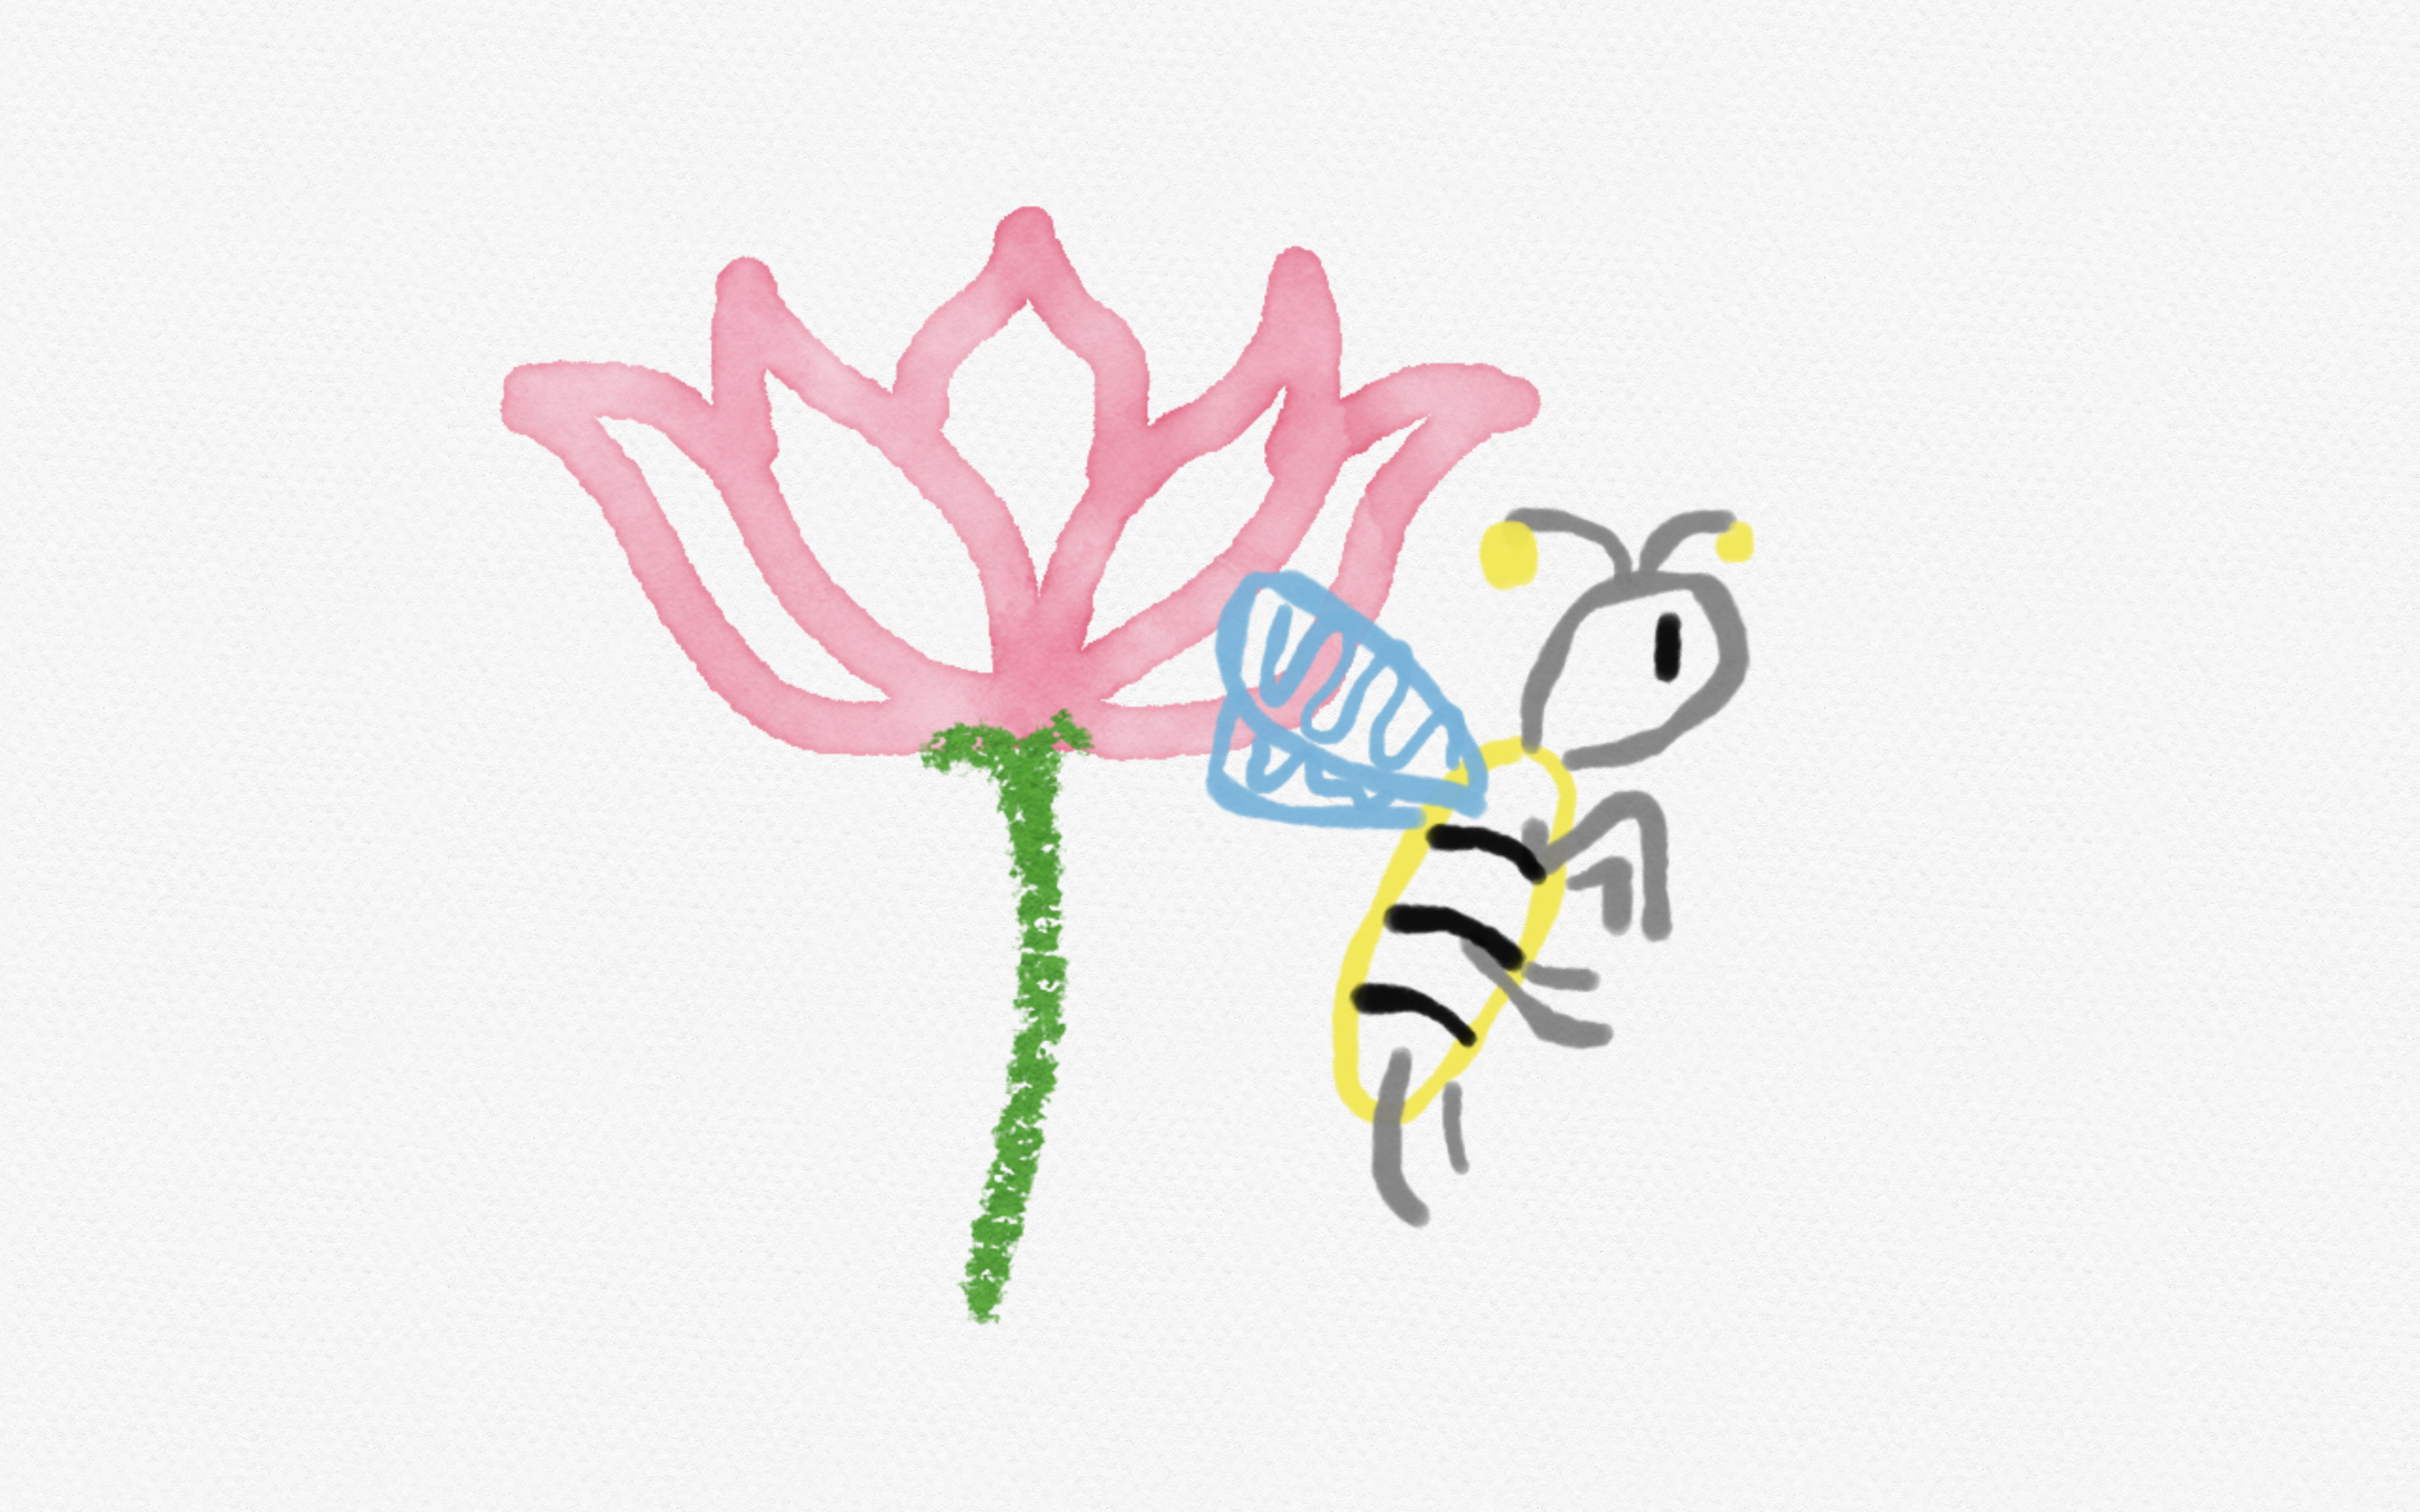
\includegraphics[width = 30em]{Logo}
\end{figure}
\newpage
\tableofcontents
\newpage

%--Einleitung--------------------------------------------------------------------------------------------------------------------------------------------------------------------------
\section{Einleitung}
\sectionauthor{Toad}
Cool text

%--Spezifikation----------------------------------------------------------------------------------------------------------------------------------------------------------------------
\section{Änderungen gegenüber der Spezifikation}
\sectionauthor{Mario}
Cool text

\subsection{Geänderte Views}
Cool list

\subsection{Paketstruktur und verwendete Klassen}
Cool list

\subsection{Datenbankschema}
Cool list

%--Implementierungsplan----------------------------------------------------------------------------------------------------------------------------------------------------------
\section{Änderungen gegenüber dem Impl'plan}
\sectionauthor{Luigi}
Cool text

\subsection{Milestone 1}
Cool table

\subsection{Milestone 2}
Cool table

\subsection{Milestone 3}
Cool table

\subsection{Allgemeine Schwierigkeiten}
Cool text

%--Metriken----------------------------------------------------------------------------------------------------------------------------------------------------------------------------
\section{Code-Metriken}
\sectionauthor{Yoshi}

Im Folgenden werden verschiedene Code-Metriken allgemein vorgestellt und für das erstellte Projekt angegeben. 
Darüber hinaus lassen sich diese Metriken in drei allgemeine Untersuchungsbereiche unterteilen: 
Allgemeine Metriken, Komplexitäts-bezogene Metriken, und Abhängigkeits-bezogene Metriken.
Durch Angabe dieser Metriken wird eine genauere Analyse des Codes aus verschiedenen Sichten ermöglicht.

\subsection{Allgemeine Metriken}

%--Table for facelets
\begin{longtable}{@{\extracolsep{\fill}}ll@{}}
\toprule
\multicolumn{2}{l}{\textbf{Facelets}} \\* \midrule
\endfirsthead
\endhead
\textbf{Anzahl Facelets} & Number \\
\textbf{Anzahl Zeilen XML Code} & Number \\* \bottomrule
\end{longtable}

%--Table for packages
\begin{longtable}{@{\extracolsep{\fill}}llll@{}}
\toprule
\multicolumn{4}{l}{\textbf{Metriken nach Paket}} \\* \midrule
\textbf{Paketname} & \textbf{\begin{tabular}[c]{@{}l@{}}Anzahl\\ Java-Zeilen\end{tabular}} & \textbf{\begin{tabular}[c]{@{}l@{}}Anzahl\\ Java-Methoden\end{tabular}} & \textbf{\begin{tabular}[c]{@{}l@{}}Anzahl\\ Java-Klassen\end{tabular}} \\* \midrule
\endfirsthead
\textbf{Paketname} & \textbf{\begin{tabular}[c]{@{}l@{}}Anzahl\\ Java-Zeilen\end{tabular}} & \textbf{\begin{tabular}[c]{@{}l@{}}Anzahl\\ Java-Methoden\end{tabular}} & \textbf{\begin{tabular}[c]{@{}l@{}}Anzahl\\ Java-Klassen\end{tabular}} \\* \midrule
\endhead
Input	 & Input & Input & Input \\
Input	 & Input & Input & Input \\* \bottomrule
\end{longtable}

\subsection{Komplexitäts-bezogene Metriken}

%--Table for packages
\begin{longtable}{@{\extracolsep{\fill}}llll@{}}
\toprule
\multicolumn{4}{l}{\textbf{Metriken nach Paket}} \\* \midrule
\textbf{Paketname} & \textbf{Durchschnittliche zyklomatische Komplexität*} \\* \midrule
\endfirsthead
\textbf{Paketname} & \textbf{Durchschnittliche zyklomatische Komplexität} \\* \midrule
\endhead
Input	 & Input \\
Input	 & Input \\* \bottomrule
\end{longtable}

%--Table for methods
\begin{longtable}{@{\extracolsep{\fill}}ll@{}}
\toprule
\multicolumn{2}{l}{\textbf{Die 10 komplexeste Methoden nach kognitiver Komplexität}} \\* \midrule
\textbf{Methodenname} & \textbf{Kognitive Komplexität*} \\* \midrule
\endfirsthead
\textbf{Methodenname} & \textbf{Kognitive Komplexität} \\* \midrule
\endhead
Input	 & Input \\
Input	 & Input \\* \bottomrule
\end{longtable}

\paragraph{Zyklomatische Komplexität} 
Als zyklomatische Komplexität bezeichnet man die maximale Anzahl an Pfaden im entsprechenden Kontroll-Fluss Grahpen, die sich jeweils im Vergleich zu allen anderen Pfaden in der Menge an besuchten Knoten um mindestens einen unterscheiden. 

\paragraph{Kognitive Komplexität} 
Im Code setzt sich die Metrik zur kognitiven Komplexität aus der Anzahl an Brüchen im Kontrollfluss und Verschachtelungen von entsprechenden Kontrollflussanweisungen zusammen. 
Im Gegensatz zur zyklomatischen Komplexität fasst diese Metrik die Schwierigkeit, mit der das gegebene Code zum Lesen und Verstehen ist.

\subsection{Abhängigkeits-bezogene Metriken}

%--Table for packages
\begin{longtable}{@{\extracolsep{\fill}}lll@{}}
\toprule
\multicolumn{3}{l}{\textbf{Metriken nach Paket}} \\* \midrule
\textbf{Paketname} & \textbf{\begin{tabular}[c]{@{}l@{}}Anzahl\\ Paket-\\Abhängigkeiten\end{tabular}} & \textbf{\begin{tabular}[c]{@{}l@{}}Anzahl Paketen\\ mit dieser\\ Abhängigkeit\end{tabular}} \\* \midrule
\endfirsthead
\textbf{Paketname} & \textbf{\begin{tabular}[c]{@{}l@{}}Anzahl\\ Paket-\\Abhängigkeiten\end{tabular}} & \textbf{\begin{tabular}[c]{@{}l@{}}Anzahl Paketen\\ mit dieser\\ Abhängigkeit\end{tabular}} \\* \midrule
\endhead
Input	 & Input & Input \\
Input	 & Input & Input \\* \bottomrule
\end{longtable}

%--Reference--------------------------------------------------------------------------------------------------------------------------------------------------------------------------
\section{Reference}
\sectionauthor{Wario}
Cool text

\subsection{Nice looking table}
\begin{longtable}{@{\extracolsep{\fill}}lllll@{}}
\toprule
\textbf{Header 1} & \textbf{Header 2} & \textbf{Header 3} & \textbf{Header 4} & \textbf{Header 5} \\* \midrule
\endfirsthead
%
\endhead
%
Text 1            & Text 2            & Text 3            & Text 4            & Text 5            \\
Text 1            & Text 2            & Text 3            & Text 4            & Text 5            \\* \bottomrule
\end{longtable}

\subsection{Nice looking landscape-table}
\begin{landscape}
\begin{longtable}{@{\extracolsep{\fill}}lllll@{}}
\toprule
\textbf{Header 1} & \textbf{Header 2} & \textbf{Header 3} & \textbf{Header 4} & \textbf{Header 5} \\* \midrule
\endfirsthead
%
\endhead
%
Text 1            & Text 2            & Text 3            & Text 4            & Text 5            \\
Text 1            & Text 2            & Text 3            & Text 4            & Text 5            \\* \bottomrule
\end{longtable}
\end{landscape}

\end{document}
